\documentclass[fleqn]{jsarticle}

\usepackage{graphicx}
\usepackage{amsmath,amssymb}
\usepackage{amsmath}
\usepackage{fancyhdr}

\pagestyle{fancy}
\fancyhead[RE,RO]{先端データ解析論 レポート}

\usepackage{xcolor}
\usepackage[justification=centering]{caption}
\usepackage{listings}
\renewcommand{\lstlistingname}{リスト}
\lstset{language=Python,%
        % basicstyle=\footnotesize,%
        basicstyle=\tiny,%
        commentstyle=\textit,%
        classoffset=1,%
        keywordstyle=\bfseries,%
      	frame=tRBl,framesep=5pt,%
      	showstringspaces=false,%
        linewidth=38em,
      	}%

\begin{document}

\newcommand{\argmax}{\mathop{\rm argmax}\limits}
\newcommand{\argmin}{\mathop{\rm argmin}\limits}

\title{先端データ解析論 第7回レポート}
\author{電子情報学専攻 48-176403 石毛真修}
\maketitle


\section*{大問1.}
ガウスカーネルモデルを用いた、最小二乗確率的分類の実装
\begin{center}
\begin{tabular}{c}
  \begin{lstlisting}[]
    import numpy as np
    from numpy.random import randn
    from matplotlib import pyplot


    class DataGenerator:
      def __init__(self, n=90, c=3):
          assert(n % c == 0)
          length = n // c
          self._classes = np.arange(1, c + 1)
          self._y = np.array([np.ones(length) * i for i in range(1, c + 1)])
          self._x = randn(c, length) + np.array([np.linspace(-3, 3, c)] * length).T

      @property
      def x_1d(self):
          return self._x.reshape(-1)

      @property
      def y_1d(self):
          return self._y.reshape(-1)

      @property
      def classes(self) -> list:
          return list(self._classes)


    class GauseKernelRegression:
      H = .2
      LAMBDA = .1

      def __init__(self, data: DataGenerator):
          self._data = data
          self._K = self._build_K(data.x_1d)
          self._thetas = dict.fromkeys(data.classes, None)

      def _kernel(self, x: np.array, c: np.array) -> np.array:
          diff = np.abs(x - c)
          return np.exp(- diff**2 / (2 * self.H**2))

      def _build_K(self, X: np.array) -> np.array:
          return np.array([self._line_kernel(v) for v in X])

      def _line_kernel(self, v: float) -> np.array:
          vec = np.ones(self._data.x_1d.shape) * v
          return self._kernel(vec, self._data.x_1d)

      def _theta(self, label: int) -> np.array:
          if self._thetas[label] is not None:
              return self._thetas[label]
          else:
              Q = self._K.T @ self._K + self.LAMBDA * np.identity(len(self._data.x_1d))
              inv_Q = np.linalg.inv(Q)
              th = inv_Q @ self._K.T @ (self._data.y_1d == label)
              self._thetas[label] = th
              return th

      def _psudo_prob(self, x: float, y: int) -> float:
          return self._line_kernel(x) @ self._theta(y)

      def probs(self, x: float) -> np.array:
          ps = np.array([max(0, self._psudo_prob(x, y)) for y in self._data.classes])
          return ps / np.sum(ps)

          data = DataGenerator(n=90, c=3)
          gkr = GauseKernelRegression(data)
  \end{lstlisting}
\end{tabular}{c}
\end{center}

\begin{center}
  \begin{tabular}{c}
  \begin{lstlisting}[]

    # Create Data and plot
    N = 100
    X = np.linspace(-5, 5, N)
    probs = np.array([gkr.probs(x) for x in X])

    axes = plt.gca()
    axes.set_xlim([-5, 5])
    axes.set_ylim([-.5, 1.5])

    plt.plot(X, probs[:, 0], 'b')
    plt.plot(X, probs[:, 1], 'r--')
    plt.plot(X, probs[:, 2], 'g|')

    plt.plot(data._x[0], -.1 * np.ones(data._x.shape[1]), 'bo')
    plt.plot(data._x[1], -.2 * np.ones(data._x.shape[1]), 'rx')
    plt.plot(data._x[2], -.1 * np.ones(data._x.shape[1]), 'gv')

  \end{lstlisting}
\end{tabular}{c}
\end{center}

実行すると次のような結果を得る.
\begin{figure}[h]
  \begin{center}
    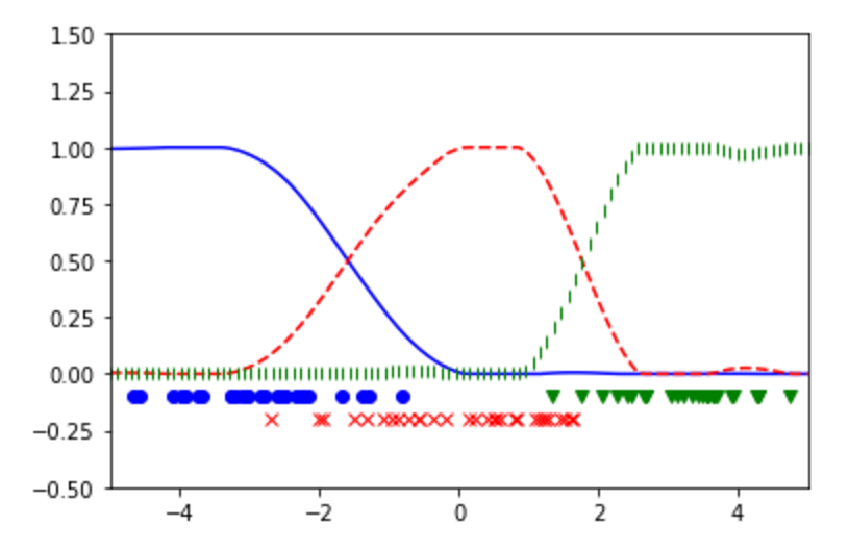
\includegraphics[width=0.6\textwidth]{figs/LogisticRegression.eps}
  \end{center}
  \caption{ガウスカーネルモデルによる最小自乗確率的分類の結果}
\end{figure}

\newpage

\section*{大問2.}
\begin{eqnarray*}
  B_\tau(y) = \sum^c_{y^{(\tau+1)},..., y^{(m_i)}=1} exp\left(
    \sum^{m_i}_{k=\tau+2} {\mathbf \zeta}^{\mathrm T} {\mathbf \varphi}({\mathbf x}^{(k)}_i, y^{(k)}, y^{(k-1)})
      + {\mathbf \zeta}^{\mathrm T} {\mathbf \varphi} ({\mathbf x}^{(\tau+1)}_i, y^{(\tau+1)}, y^{(\tau)})
    \right)
\end{eqnarray*}
を次のような再帰的な表現に変形する。
\begin{eqnarray*}
  B_\tau(y^{(\tau)}) = \sum^c_{y^{(\tau+1)}=1} B_{\tau+1}(y^{(\tau+1)}) exp\left(
    {\mathbf \zeta}^{\mathrm T} {\mathbf \varphi} ({\mathbf x}^{(\tau+1)}_i, y^{(\tau+1)}, y^{(\tau)})
  \right)
\end{eqnarray*}


\subsection*{証明}
\begin{eqnarray*}
  B_\tau(y^{(\tau)}) &=& \sum^c_{y^{(\tau+1)},..., y^{(m_i)}=1} exp\left(
      \sum^{m_i}_{k=\tau+2} {\mathbf \zeta}^{\mathrm T} {\mathbf \varphi}({\mathbf x}^{(k)}_i, y^{(k)}, y^{(k-1)})
      + {\mathbf \zeta}^{\mathrm T} {\mathbf \varphi} ({\mathbf x}^{(\tau+1)}_i, y^{(\tau+1)}, y^{(\tau)})
    \right)\\
  &=& \sum^c_{y^{(\tau+1)}=1} \sum^c_{y^{(\tau+2)},..., y^{(m_i)}=1} exp\left(
      \sum^{m_i}_{k=\tau+3} {\mathbf \zeta}^{\mathrm T} {\mathbf \varphi}({\mathbf x}^{(k)}_i, y^{(k)}, y^{(k-1)})
      + {\mathbf \zeta}^{\mathrm T} {\mathbf \varphi} ({\mathbf x}^{(\tau+1)}_i, y^{(\tau+1)}, y^{(\tau)}) \right)\\
      &&\hspace{20em} exp\left( {\mathbf \zeta}^{\mathrm T} {\mathbf \varphi}({\mathbf x}^{(\tau+1)}_i, y^{(\tau+1)}, y^{(\tau)} \right)\\
  &=& \sum^c_{y^{(\tau+1)}=1} B_{\tau+1}(y^{(\tau+1)})
      exp\left( {\mathbf \zeta}^{\mathrm T} {\mathbf \varphi}({\mathbf x}^{(\tau+1)}_i, y^{(\tau+1)}, y^{(\tau)} \right)
\end{eqnarray*}

\newpage

\section*{大問3.}
\begin{eqnarray*}
  P_\tau(y) = \max_{y^{(1)},..., y^{(\tau-1)} \in \{1,...,c\}} \left[
    \sum^{\tau-1}_{k=1} \hat{\mathbf \zeta}^{\mathrm T} {\mathbf \varphi}({\mathbf x}^{(k)}_i, y^{(k)}, y^{(k-1)})
      + \hat{\mathbf \zeta}^{\mathrm T} {\mathbf \varphi} ({\mathbf x}^{(\tau)}_i, y^{(\tau)}, y^{(\tau-1)})
    \right]
\end{eqnarray*}
を次のような再帰的な表現に変形する。
\begin{eqnarray*}
  P_\tau(y^{(\tau)}) = \max_{y^{(\tau-1)} \in \{1,...,c\}} \left[
    P_{\tau-1}(y^{(\tau-1)}) +
    {\mathbf \zeta}^{\mathrm T} {\mathbf \varphi} ({\mathbf x}^{(\tau)}_i, y^{(\tau)}, y^{(\tau-1)})
  \right]
\end{eqnarray*}


\subsection*{証明}
\begin{eqnarray*}
  P_\tau(y) &=& \max_{y^{(1)},..., y^{(\tau-1)} \in \{1,...,c\}} \left[
    \sum^{\tau-1}_{k=1} \hat{\mathbf \zeta}^{\mathrm T} {\mathbf \varphi}({\mathbf x}^{(k)}_i, y^{(k)}, y^{(k-1)})
    + \hat{\mathbf \zeta}^{\mathrm T} {\mathbf \varphi} ({\mathbf x}^{(\tau)}_i, y^{(\tau)}, y^{(\tau-1)}) \right]\\
  &=& \max_{y^{(\tau-1)} \in \{1,...,c\}} \left[
    \hat{\mathbf \zeta}^{\mathrm T} {\mathbf \varphi} ({\mathbf x}^{(\tau)}_i, y^{(\tau)}, y^{(\tau-1)}) \right.\\
      && \left. + \max_{y^{(1)},..., y^{(\tau-2)} \in \{1,...,c\}} \left[
      \sum^{\tau-1}_{k=1} \hat{\mathbf \zeta}^{\mathrm T} {\mathbf \varphi}({\mathbf x}^{(k)}_i, y^{(k)}, y^{(k-1)})
      \hat{\mathbf \zeta}^{\mathrm T} {\mathbf \varphi} ({\mathbf x}^{(\tau-1)}_i, y^{(\tau-1)}, y^{(\tau-2)})
      \right] \right]\\
  &=& \max_{y^{(\tau-1)} \in \{1,...,c\}} \left[
    P_{\tau-1}(y^{(\tau-1)}) +
    {\mathbf \zeta}^{\mathrm T} {\mathbf \varphi} ({\mathbf x}^{(\tau)}_i, y^{(\tau)}, y^{(\tau-1)})
    \right]
\end{eqnarray*}









\newpage



\end{document}
